\chapter{Markov Chain}

In Earth Science, we often look at the time evolution of some variables, like temperature, rainfall etc. Sometimes, the variables can be modelled as random variables. A simple daily example will be tossing a coin (no matter it is fair or not), where the outcomes (head/tail) are probabilistic. Some Earth System examples are the chances of extreme weathers, or some slow geological processes. Such processes involving random variables are known as \textit{Stochastic Processes}, and we will visit the related Statistical concepts. Particularly, we will investigate the so-called \textit{Markov Chain}, which assumes the present state of a stochastic process only depends on the past. Modelling a stochastic process with Markov Chain can give more satisfactory results when it is believed that the process inherently correlates strongly with previous states, or is said to be have \textit{memory}.

\section{Basic Statistical Ideas for Markov Chain}

\subsection{Lagged Auto-correlation}

First, let's talk about how we determine if a time-series possesses some sorts of memory. Memory causes the past of a time-series to influence the present, and hence will leave a mark when we try to correlate the past and the present of the time-series. Here comes the idea of \textit{Lagged Auto-correlation}, which is the correlation between a time-series and itself, but one of them is lagged and shifted by a certain amount of days, $k$ (The direction of shifting does not matter much, and we only care about the overlapping part), and it is more specifically known as the \textit{Lag-k Auto-correlation}.

\begin{defn}
\label{1403}
The lag-k auto-correlation $r_k$ of a time-series $\{x\}$ is defined as
\begin{align*}
r_k &= \frac{\sum_{i=1}^{n-k}(x_i - \bar{x}_{-})(x_{i+k} - \bar{x}_{+})}{\sqrt{(\sum_{i=1}^{n-k}(x_i - \bar{x}_{-})^2) (\sum_{i=k+1}^{n}(x_i - \bar{x}_{+})^2)}}
\end{align*}
where $\{x_{-}\}$ and $\{x_{+}\}$ denotes the sequence representing the earliest and latest $n-k$ data. An overline denotes an average. Alternatively, the formula can be written as
\begin{align*}
r_k &= \frac{\text{Cov}(\{x_{-}\},\{x_{+}\})}{\sqrt{\text{Var}(\{x_{-}\}) \text{Var}(\{x_{+}\})}} \\
&= \frac{\text{Cov}(\{x_{-}\},\{x_{+}\})}{\sqrt{\text{Cov}(\{x_{-}\}, \{x_{-}\}) \text{Cov}(\{x_{+}\}, \{x_{+}\})}}
\end{align*}
where the definitions of variance and covariance are those from definitions \ref{variance} and \ref{covariance}.
\end{defn}
If the lag-k auto-correlation of a time-series is close to $1$ or $-1$, it means that the state at a certain time will probably lead to a similar/opposite state $k$ time steps later.

\begin{exmp}
For the traffic flow data over some seven days of a highway below, find its lag-1 auto-correlation.
\begin{center}
\begin{tabular}{|c|c|c|c|c|c|c|c|}
\hline
Day & 1 & 2 & 3 & 4 & 5 & 6 & 7 \\
\hline
Vehicles per Hour & 680 & 820 & 760 & 790 & 840 & 1030 & 1080 \\
\hline
\end{tabular}
\end{center}
We first locate the first and last $7-1 = 6$ data as two smaller time-series, which are $\{x_-\} = \{680, 820, 760, 790, 840, 1030\}$ and $\{x_+\} = \{820, 760, 790, 840, 1030, 1080\}$. The sample variances of the two time-series are
\begin{align*}
\text{Cov}(\{x_-\}) &= 13720 \text{ (Vehicles per Hour)}^2 \\
\text{Cov}(\{x_+\}) &= 17987 \text{ (Vehicles per Hour)}^2
\end{align*}
and their sample covariance is
\begin{align*}
\text{Cov}(\{x_{-}\},\{x_{+}\}) &= 12000 \text{ (Vehicles per Hour)}^2
\end{align*}
The readers are encouraged to verify the numbers. Hence by the formula above, the lag-1 auto-correlation is
\begin{align*}
r_1 &= \frac{12000}{\sqrt{13720*17987}} = 0.7639
\end{align*}
It means that a busy traffic will likely be followed by a more or less busy traffic the next day, which is not unreasonable.\\
Short Exercise: Compute the lag-2 auto-correlation.
\end{exmp}

\subsection{Conditional Probabilities, Stochastic Matrices}
To fully understand Markov Chain, we also need to know what conditional probabilities are. The \textit{Conditional Probability} $P(A|B)$ is the probability of event $A$ occurring given event $B$ has occurred. For an evolving system which has a finite amount of states and can only possesses one state at a time, e.g. on-and-off, the conditional probability $P(A_i^{[k+1]}|A_j^{[k]})$ represents the probability of state $A_i$ occurring at time step $k+1$ if the state is $A_j$ at time step $k$. An Atmospheric Science example is daily weather reports, which in a simplistic sense, can be sunny, rainy, windy. If it is rainy today, then there is a relatively high chance it is rainy tomorrow, i.e. $P(\text{rainy}^{[k+1]}|\text{rainy}^{[k]})$ is high.\\
\\
For $N$ finite, distinct events in a well-defined, closed system, so that the system always take one and only one of the events as its state, we have the following observation.
\begin{thm}
The sum of conditional probabilities for a changing system with $N$ mutually exclusive (only one state at a time) and exhaustive (the states cover all possibilities) events $A_1, A_2, \cdots, A_N$, we have
\begin{align*}
\sum_{i=1}^N P(A_i^{[k+1]}|A_j^{[k]}) &= P(A_1^{[k+1]}|A_j^{[k]}) + P(A_2^{[k+1]}|A_j^{[k]}) + \cdots + P(A_N^{[k+1]}|A_j^{[k]}) \\
&= 1
\end{align*}
where $k$ denotes a particular time step. It means that any given event $A_j$ must consequently lead to one of possible states (including $A_j$ itself) at the next time step.
\end{thm}
As a result, we can express conditional probabilities $P(A_i^{[k+1]}|A_j^{[k]})$ for a particular $A_j$ in a system using a column vector with entries that sum up to $1$. Using daily weather as an example, assumed there are only three states (sunny/windy/rainy), if a sunny day has a chance of $0.8$ to be followed by another sunny day, and $0.15$/$0.05$ for another windy/rainy day. Then we can write
\begin{center}
\begin{tabular}{|c|c|}
\hline
k+1 $\backslash$ k & Sunny \\
\hline
Sunny & 0.8 \\
\hline
Windy & 0.15 \\
\hline 
Rainy & 0.05 \\
\hline
\end{tabular}
\end{center}
as a column vector
\begin{align*}
\begin{bmatrix}
0.8 \\
0.15 \\
0.05
\end{bmatrix}
\end{align*}
We can do the same for the other two states. If a windy day has a probability of $0.2$/$0.5$/$0.3$ leading to a sunny/windy/rainy day, and a rainy day has a chance of $0.1$/$0.2$/$0.7$ leading to a sunny/windy/rainy day, then
\begin{center}
\begin{tabular}{|c|c|c|c|}
\hline
k+1 $\backslash$ k & Sunny & Windy & Rainy \\
\hline
Sunny & 0.8 & 0.2 & 0.1\\
\hline
Windy & 0.15 & 0.5 & 0.2 \\
\hline 
Rainy & 0.05 & 0.3 & 0.7 \\
\hline
\end{tabular}
\end{center}
can be summarized by the so-called \textit{Stochastic Matrix} as
\begin{align*}
P = 
\begin{bmatrix}
0.8 & 0.2 & 0.1\\
0.15 & 0.5 & 0.2 \\
0.05 & 0.3 & 0.7
\end{bmatrix}
\end{align*}
\begin{defn}
\label{1401}
The stochastic matrix for a closed system with mutually exclusive and exhaustive events $A_1, A_2, \cdots, A_N$, is
\begin{align*}
P =
\begin{bmatrix}
P(A_1^{[k+1]}|A_1^{[k]}) & P(A_1^{[k+1]}|A_2^{[k]}) & \cdots & P(A_1^{[k+1]}|A_N^{[k]})\\
P(A_2^{[k+1]}|A_1^{[k]}) & P(A_2^{[k+1]}|A_2^{[k]}) & & \\
\vdots & & \ddots & \\
P(A_N^{[k+1]}|A_1^{[k]}) & & & P(A_N^{[k+1]}|A_N^{[k]})
\end{bmatrix}
\end{align*}
where $P_{ij}$ is the conditional probability of moving to state $i$ at the next time step from the present state $j$.
\end{defn}
Notice that the entries along any column add up to $1$. Column $j$ holds the conditional probabilities of state $j$ leading to different states at the next time step.

\section{Markov Chain}

\subsection{State Vector, Steady State}

Processes can be represented by such stochastic matrices are called Markov Chains. It is assumed that the conditional probabilities outlined in the stochastic matrices do not change in time. Given a probability vector (or the \textit{State Vector}) $\vec{x}^{[k]}$ consisting of the probabilities of having different states at a certain time step $k$, we can calculate the probability vector $\vec{x}^{[k+1]}$ at the next time step $k+1$ as $P\vec{x}^{[k]}$.

\begin{proper}
Given a Markov Chain, with a stochastic matrix $P$ described in \ref{1401}, then the state vector $\vec{x}^{[k+1]}$ at time step $k+1$ is decided by
\begin{align*}
\vec{x}^{[k+1]} &= P\vec{x}^{[k]}   
\end{align*}
\end{proper}
\paragraph{Proof} If we look at the $i$-th entry at both sides, we have
\begin{align*}
\vec{x_i}^{[k+1]} &= P_{i1} \vec{x_1}^{[k]} + P_{i2} \vec{x_2}^{[k]} + P_{i3} \vec{x_3}^{[k]} \cdots 
\end{align*}
or more explicitly
\begin{align*}
P(A_i^{[k+1]}) &= P(A_i^{[k+1]}|A_1^{[k]}) P(A_1^{[k]}) + P(A_i^{[k+1]}|A_2^{[k]}) P(A_2^{[k]}) + \cdots \\
&= \sum_{j=1}^N P(A_i^{[k+1]}|A_j^{[k]}) P(A_j^{[k]})
\end{align*}
This result is essentially a manifestation of the \textit{Law of Total Probability}. In our circumstance, it holds as the events are mutually exclusive and exhaustive, and hence the property as well.\\
\\
Similarly, at time step $k+2$ the probability vector is $\vec{x}^{[k+2]} = P^2\vec{x}^{[k]}$. $\vec{x}^{[1]} = P\vec{x}^{[0]}, \vec{x}^{[2]} = P\vec{x}^{[1]} = P(P\vec{x}^{[0]}) = P^2\vec{x}^{[0]}, \cdots, \vec{x}^{[n]} = P^n\vec{x}^{[0]}$.

\begin{exmp}
\label{1402}
Using the previous example of weather, the stochastic matrix is
\begin{align*}
P = 
\begin{bmatrix}
0.8 & 0.2 & 0.1\\
0.15 & 0.5 & 0.2 \\
0.05 & 0.3 & 0.7
\end{bmatrix}   
\end{align*}
Find the probabilities of each type of weather occurring on Day 2, if we somehow know that the chances of being sunny/windy/rainy on Day 1 is $0.3$/$0.4$/$0.3$. \\
\\
By the formula we have just obtained, the required state vector is
\begin{align*}
\vec{x}^{[2]} &= P\vec{x}^{[1]} \\
&=
\begin{bmatrix}
0.8 & 0.2 & 0.1\\
0.15 & 0.5 & 0.2 \\
0.05 & 0.3 & 0.7
\end{bmatrix}   
\begin{bmatrix}
0.3 \\
0.4 \\
0.3
\end{bmatrix} \\
&= 0.3
\begin{bmatrix}
0.8 \\
0.15 \\
0.05
\end{bmatrix}
+ 0.4
\begin{bmatrix}
0.2 \\
0.5 \\
0.3
\end{bmatrix}
+ 0.3
\begin{bmatrix}
0.1 \\
0.2 \\
0.7
\end{bmatrix} \\
&=
\begin{bmatrix}
0.35 \\
0.305 \\
0.345
\end{bmatrix}
\end{align*}
So on Day 2, the chances of sunny/windy/rainy are $0.35$/$0.305$/$0.345$. It is emphasized in the last step that the required state vector at the next day is just the linear combination of the conditional probability column vectors, with the weighting specified by the current state vector. It is again the Law of Total Probability working.\\
Short Exercise: Find the state vector on the next day if today is windy.
\end{exmp}

For a Markov Chain which has been ongoing for a long period of time, and the initial state becomes effectively forgotten (\textit{Memoryless}), it is desirable to obtain the steady state vector which represents the probability of every state given no prior knowledge of initial state. The steady state vector $\vec{q}$ is one that remains the same for any time step. Hence we have $\vec{q} = P\vec{q} = ... = P^n\vec{q}$.\\
\\
Rearrangement gives $(I-P)q = 0$, in which the steady-state vector $\vec{q}$ corresponds to the eigenvector of $P$ when eigenvalue is $1$. $\vec{q}$ is then calculated following the usual procedure for solving the linear system and computing the eigenvector.
\begin{defn}
The steady state of a Markov Chain is simply the eigenvector of the identity matrix minus its stochastic matrix $I - P$ that corresponds to the eigenvalue of $1$, and divided by the sum of entries so that they add up to $1$.
\end{defn}

\begin{exmp}
Continuing the last example, 
\begin{align*}
P = 
\begin{bmatrix}
0.8 & 0.2 & 0.1\\
0.15 & 0.5 & 0.2 \\
0.05 & 0.3 & 0.7
\end{bmatrix}   
\end{align*}
and
\begin{align*}
I - P = 
\begin{bmatrix}
0.2 & -0.2 & -0.1\\
-0.15 & 0.5 & -0.2 \\
-0.05 & -0.3 & 0.3
\end{bmatrix}   
\end{align*}
A simple calculation reveals that the eigenvector of $I - P$ for $\lambda=1$ is $(\frac{9}{7}, \frac{11}{14}, 1)^T$. Since the probabilities have to be added up to $1$, dividing each component by the sum yields the steady state vector $\vec{q} = (\frac{18}{43}, \frac{11}{43}, \frac{14}{43})^T \approx (0.419, 0.256, 0.326)^T$, meaning that there is $41.9\% / 25.6\% / 32.6\%$ chance of having a sunny/windy/rainy day on average.
\end{exmp}

\subsection{Expected Value Problem}
For the special case in which one of the states in Markov Chain is absorbing, i.e. no outgoing pathway and the probability to remain in the node/state is 1, all pathway will eventually lead to accumulation in this particular sink. This is referred to as an \textit{Absorbing Markov Chain} and it is possible to predict the expected time needed for any state to arrive at the absorbing state.\\
\\
We can attack this problem by finding the total expected time spent in other non-absorbing nodes, which is precisely the very same quantity we want to know. At the zeroth time step, or $T=0$, the time spent in the starting node and other nodes is one and zero unit time respectively. (We can adapt for the case where the starting condition is probabilistic, e.g. $50\%$ chance in the first node and $50\%$ chance in the second node.) At $T=k$, the average time spent during the $k$-th time step in different nodes are exactly the probabilities to land on these nodes after $k$ time steps.\\
\\
Hence the idea is to add up the time staying in every non-absorbing node over every time step. Therefore, we consider the variant of the stochastic matrix in which the row and column of the absorbing state is deleted. Assume that there are three states in the absorbing Markov Chain, and its stochastic matrix is
\begin{align*}
P &= 
\begin{bmatrix}
0.2 & 0.8 & 0\\
0.7 & 0 & 0 \\
0.1 & 0.2 & 1
\end{bmatrix}
\end{align*}
The third column shows that the third node is an absorbing node. After deleting the row and column related to the absorbing state, and only looking at those non-absorbing states, we have
\begin{align*}
P_0 &= 
\begin{bmatrix}
0.2 & 0.8\\
0.7 & 0 \\
\end{bmatrix}   
\end{align*}
Assume we starts at the first node, i.e. the probability vector representing the initial state is $(1, 0)^T$ in this case, the formula to calculating the total staying time over all time steps would be
\begin{align*}
I
\begin{bmatrix}
1 \\
0
\end{bmatrix}
+
P
\begin{bmatrix}
1 \\
0
\end{bmatrix}
+
P^2
\begin{bmatrix}
1 \\
0
\end{bmatrix}
+ \cdots 
=
(1 + P_0 + P_0^2 + \cdots)
\begin{bmatrix}
1 \\
0
\end{bmatrix}
=
\begin{bmatrix}
T_1 \\
T_2
\end{bmatrix}
\end{align*}
where the first term at the left hand side is the staying time at zeroth time step, the second term is that at first time step, and so on. $T_1$ and $T_2$ will be the total expected time spent at node $1$ and $2$. We can utilize the formula of geometric sum for matrices, and generalize the formula to accommodate more states.
\begin{proper}
The expected time for a initial state in a Markov Chain to be absorbed in the sink (assumed that there is only one sink) can be inferred from the relation
\begin{align*}
\begin{bmatrix}
T_1 \\
T_2 \\
T_3 \\
\cdots
\end{bmatrix}
=
(I - P_0)^{-1}
\vec{x_0}^{[0]}
\end{align*}
where P is the associated stochastic matrix and $P_0$ is $P$ with the row and column of the absorbing state taken away. $\vec{x_0}^{[0]}$ is the initial state vector, also with the entry corresponding to the absorbing node removed. The required expected absorption time is the sum of $T_i$, over all possible $i$. 
\end{proper}
The only caveat is that the formula of geometric sum for matrices may not be true, just like the original formula for numbers will fail if the common ratio has a magnitude larger than or equal to $1$. However, it is guaranteed for a well-behaved stochastic matrix without isolated loops, $(I - P_0)^{-1} = 1 + P_0 + P_0^2 + \cdots$ indeed holds.
\begin{exmp}
For the absorbing Markov Chain we have been discussing about, which has
\begin{align*}
P_0 &= 
\begin{bmatrix}
0.2 & 0.8\\
0.7 & 0 \\
\end{bmatrix}   
\end{align*}
We have
\begin{align*}
I - P_0 &= 
\begin{bmatrix}
0.8 & -0.8\\
-0.7 & 1 \\
\end{bmatrix} \\
(I - P_0)^{-1} &= 
\begin{bmatrix}
4.166 & 3.333 \\
2.917 & 3.333
\end{bmatrix} \\
(I - P_0)^{-1}\vec{x_0}^{[0]} &= 
\begin{bmatrix}
4.166 & 3.333 \\
2.917 & 3.333
\end{bmatrix}
\begin{bmatrix}
1 \\
0
\end{bmatrix} 
=
\begin{bmatrix}
4.166 \\
2.917
\end{bmatrix}
\end{align*}
Hence the expected time required to reach the third node starting from the first node will be just the sum of the first column in $P_0$, $4.166 + 2.917 = 7.083$.\\
Short Exercise: Find the expected time required to reach the third node if it has $50\%/50\%$ chances to start at the first/second node instead.
\end{exmp}

\subsection{Auto-correlation Predicted by Markov Chain}

The last topic we will touch about Markov Chain is its inherent auto-correlation. Consider the simplest case, where a Markov Chain only has two possible states, with a $2 \times 2$ stochastic matrix, having the form
\begin{align*}
P = 
\begin{bmatrix}
P_{11} & P_{12} \\
P_{21} & P_{22}
\end{bmatrix}
\end{align*}
Assume the first/second state represents a value of $1$/$0$ without the loss of generality. The theoretical lag-1 auto-correlation between the binary states, predicted by the Markov Chain, is definition \ref{1403} modified appropriately, that is
\begin{align*}
r_1 &= \frac{\text{Cov}(\{x_{-}\},\{x_{+}\})}{\sqrt{\text{Var}(\{x_{-}\}) \text{Var}(\{x_{+}\})}} \\
&= \frac{E(X_{-}X_{+}) - E(X_{-})E(X_{+})}{\sqrt{(E(X_{-}^2) - (E(X_{-}))^2)(E(X_{+}^2) - (E(X_{+}))^2)}}
\end{align*}
where we have used the short-cut formula for variance and covariance listed in section \ref{variancesec}. If the Markov Chain operates for a long enough time, then the average of the two time-series lagged by a day will be equal, implying that
\begin{align*}
E(X_{-}) = E(X_{+}) &= q_1
\end{align*}
where $\vec{q}$ is the stationary state vector, with $q_1$ being the stationary probability of being in state $1$. Similarly, we have
\begin{align*}
E(X_{-}^2) = E(X_{+}^2) &= q_1    
\end{align*}
since the square of an individual $1$/$0$ time-series will return itself. The remaining job is to determine $E(X_{-}X_{+})$, which is simply
\begin{align*}
E(X_{-}X_{+}) &= P(x_{+}=1 \text{ and } x_{-}=1) \\
&= P(x_{+}=1|x_{-}=1) P(x_{-}=1) \\
&= P_{11} q_1
\end{align*}
So the lag-1 auto-correlation is
\begin{align*}
r_1 &= \frac{(P_{11}q_1-q_1^2)}{\sqrt{(q_1-q_1^2)(q_1-q_1^2)}} \\
&= \frac{q_1(P_{11}-q_1)}{(q_1-q_1^2)} \\
&= \frac{P_{11}-q_1}{1-q_1}
\end{align*}
But, by the eigenvector definition of the stationary state, we have
\begin{align*}
P_{11}q_1 + P_{12}q_2 &= q_1 \\
P_{11}q_1 + P_{12}(1-q_1) &= q_1 \\
(1 - P_{11} + P_{12}) q_1 &= P_{12}
\end{align*}
Substituting this into the formula of lag-1 auto-correlation, we arrive at
\begin{align*}
r_1 &= \frac{(1 - P_{11} + P_{12})(P_{11}-q_1)}{(1 - P_{11} + P_{12})(1-q_1)} \\
&= \frac{P_{11}(1 - P_{11} + P_{12}) - (1 - P_{11} + P_{12})q_1}{1 - P_{11} + P_{12} - (1 - P_{11} + P_{12})q_1} \\
&= \frac{P_{11}(1 - P_{11} + P_{12}) - P_{12}}{1 - P_{11} + P_{12} - P_{12}} \\
&= \frac{(1-P_{11})(P_{11}-P_{12})}{1 - P_{11}} \\
&= P_{11} - P_{12}
\end{align*}
Therefore, the magnitude of lag-1 auto-correlation estimated from Markov Chain is simply the difference between the two conditional probabilities on the same row in the stochastic matrix. By the same essence, the lag-k auto-correlation can be inferred from $r_k = Q_{11} - Q_{12}$, where $Q = P^k$. Fortunately, due to the structure of stochastic matrix, we have a very simple formula for lag-k auto-correlation, which is just the $k$-th power of the lag-1 auto-correlation, $r_k = r_1^k$.

\begin{proper}
The lag-k auto-correlation of a binary Markov Chain, with a stochastic matrix $P$, is
\begin{align*}
r_k = (P^k)_{11} - (P^k)_{12} = (P_{11} - P_{12})^k = r_1^k
\end{align*}
\paragraph{Proof} The formula holds for $k=1$ as we just see, now we will briefly prove the equality for $k = 2$.
\begin{align*}
P^2 &=
\begin{bmatrix}
P_{11} & P_{12} \\
P_{21} & P_{22} \\
\end{bmatrix}^2 \\
&= 
\begin{bmatrix}
P_{11} & P_{12} \\
1-P_{11} & 1-P_{12} \\
\end{bmatrix}
\begin{bmatrix}
P_{11} & P_{12} \\
1-P_{11} & 1-P_{12} \\
\end{bmatrix} \\
&=
\begin{bmatrix}
P_{11}^2 - P_{12}(1-P_{11}) & P_{11}P_{12} - P_12(1-P_{12}) \\
\cdots & \cdots \\
\end{bmatrix}
\end{align*}
So
\begin{align*}
(P^2)_{11} - (P^2)_{12} &= (P_{11}^2 - P_{12}(1-P_{11})) -  (P_{11}P_{12} - P_12(1-P_{12})) \\
&= P_{11}^2 - 2P_{11}P_{12} + P_{12}^2 \\
&= (P_{11} - P_{12})^2
\end{align*}
as we have asserted. Cases for $k \geq 3$ can be proved via Mathematical Induction.
\end{proper}
For instance, given a two-state Markov Chain with the stochastic matrix
\begin{align*}
P = 
\begin{bmatrix}
0.35 & 0.75 \\
0.65 & 0.25
\end{bmatrix}
\end{align*}
The lag-1 auto-correlation will be $0.35 - 0.75 = 0.25 - 0.65 = -0.4$, and the lag-4 auto-correlation will be $(-0.4)^4 = 0.0256$. Lag-k auto-correlation of any Markov Chain always decays exponentially.

\section{Exercise}

\begin{Exercise}
For the island Gu-Nei-Ng-Dou, if it is a sunny day, then the next day has $75\%$ chance of being sunny, $10\%$ chance of being windy, and $15\%$ of being rainy. Meanwhile, a windy day has $60\%$/$25\%$/$15\%$ chance leading to a sunny/windy/rainy day, and a rainy day has $30\%$/$20\%$/$50\%$ chance leading to a sunny/windy/rainy day. Find:
\begin{enumerate}[label=(\alph*)]
\item the probability of getting a rainy day three days after a rainy day,
\item the steady-state probability of all three types of weather,
\item the probability of getting at least one sunny day today and tomorrow if it is sunny yesterday.
\end{enumerate}
\end{Exercise}

\begin{Exercise}
Not all stochastic matrices are well-behaved (or formally, regular) Markov Chains. Consider the case where there exists three states, A, B, and C. State A always lead to state B, which in turn always lead to state C, and state C will always move back to state A. Construct the stochastic matrix for this case, and find its steady-state vector. Despite the existence of a steady-state vector, prove that it is an unstable, oscillating system by a counter-example, as well as an intuitive argument.
\end{Exercise}

\begin{Exercise}
For the carbon cycle below, calculate the rate constant $k$ for each transport process, and verify that on average it takes about 213000 years for carbon in the ocean reservoir to be buried in the sediment by (a) absorbing Markov Chain, (b) considering the biosphere-atmosphere-ocean as a single reservoir and calculating the lifetime $\tau = \frac{1}{k} = \frac{\text{total stock mass}}{\text{flux}}$. Also, if the pathway to sediment is neglected, find the steady-state vector of the biosphere-atmosphere-ocean system and confirm they are already in steady state as one would expect.
\begin{center}
\fbox{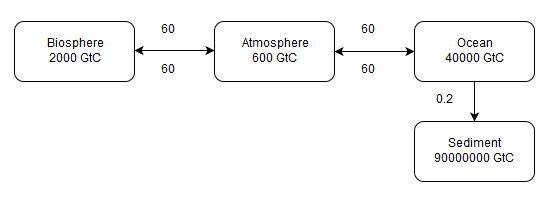
\includegraphics[scale = 0.5]{carboncycle.jpg}}
\end{center}
\end{Exercise}

\begin{Exercise}
Aftershocks can happen when an earthquake or another aftershock has occurred. Assume that the probability of aftershocks (rows) can be modelled such that it depends on the prior earthquake/aftershock only (columns), as the table shown below. Find the expected total number of earthquakes/aftershocks if there is an earthquake of magnitude 8.
\begin{center}
\begin{tabular}{|c|c|c|c|c|}
\hline
& M8 & M6-7 & M$\leq$5 & Stops\\
\hline
M8 & 0.1 & 0 & 0 & 0\\
\hline
M6-7 & 0.8 & 0.66 & 0 & 0\\
\hline
M$\leq$5 & 0.1 & 0.32 & 0.92 & 0\\
\hline
Stops & 0 & 0.02 & 0.08 & 1\\
\hline
\end{tabular}
\end{center}
Note: The numbers are made up and the real-world situation is much more complicated. Markov Chain can definitely be a tool for Seismology, but the usage will be more involved.
\end{Exercise}

\begin{Exercise}
Daniel is drunk at a bar. He wants to go to the train station so that he can go home. However, since he is drunk, he loses his sense of direction, and will move randomly along the green edge (shown in the map below) once at a time. Assume that at any starred location, the chances of moving to all other neighbouring locations are equal. Nevertheless, once he arrives at the train station, he will stop wandering and take the train. How many moves does it take on average for Daniel to reach the train station?
\begin{center}
(Placeholder for Diagram)
\end{center}
\end{Exercise}

\begin{Exercise}
Attempt \href{https://projecteuler.net/problem=84}{Project Euler Problem 84}, preferably with programming.
\end{Exercise}